\chapter{Datasets and Experimental Protocol}
\label{chap:datasets}
\chaptermark{Datasets and protocol}

% Draft requested by the author on 2026-11-06. Dataset counts are computed
% from the released files, not inferred from benchmark tables. See journal.
This chapter defines the data and experimental procedures used to reproduce
TranAD+ and study its simplification. Dataset properties are separated from
choices made in the implementation. This distinction is necessary because a
change in preprocessing, score construction or evaluation can change a metric
without changing the trained network.

The same reconstruction principle is applied to the three main datasets, but
the available annotations differ. We therefore distinguish the model output,
which is an error for each evaluated sample, from the unit on which detection
is assessed. We also separate evaluations that use test labels to optimize a
score from scoring settings selected on validation data and subsequently
applied to test fragments.

\section{Dataset selection and roles in the study}
\label{sec:datasets-roles}
The experimental work has two related purposes. The first is to reconstruct
the reference results on the six datasets considered in the TranAD+
paper~\cite{Yermakov2025TranADPlus}. The second is to investigate model cost
and detection performance on a smaller set relevant to spacecraft telemetry.
The datasets and their roles are listed in Table~\ref{tab:datasets-roles}.

\begin{table}[htbp]
  \centering
  \small
  \begin{tabularx}{\textwidth}{@{}lXX@{}}
    \toprule
    Dataset & Data source & Role in this thesis \\
    \midrule
    \acs{OPS-SAT} & Satellite telemetry fragments & Reference application and main simplification study \\
    \acs{SMAP} & Earth-observation satellite telemetry and command inputs & Benchmark reproduction and main simplification study \\
    \acs{MSL} & Mars rover telemetry and command inputs & Benchmark reproduction and main simplification study \\
    \acs{SMD} & Server operating measurements & Benchmark reproduction \\
    SWaT & Water-treatment testbed & Benchmark reproduction \\
    WADI & Water-distribution testbed & Benchmark reproduction \\
    DSN\_1k & Deep Space Network communications monitoring & Benchmark reproduction \\
    \bottomrule
  \end{tabularx}
  \caption{Dataset roles. The six reproduction datasets follow the scope of
  the TranAD+ paper. The main model study uses \acs{OPS-SAT}, \acs{SMAP} and
  \acs{MSL}; their descriptions follow the respective dataset sources.}
  \label{tab:datasets-roles}
\end{table}

\ac{OPS-SAT} is the reference application because its data were collected
on an operational experimental satellite and annotated by spacecraft
operations engineers~\cite{Ruszczak2025OPSSAT}. \ac{SMAP} and \ac{MSL}
provide additional spacecraft telemetry benchmarks already used by
TranAD+~\cite{Hundman2018Spacecraft,Yermakov2025TranADPlus}. \ac{SMAP} is an
Earth-orbiting satellite; \ac{MSL} is the Curiosity rover on Mars. Their common
relevance is spacecraft monitoring, rather than identical platforms,
sensors or operating conditions.

The additional reproduction datasets help assess the reference implementation
across the domains used in the published comparison. They are not included
in the main architecture grid. Their benchmark-specific configurations and
preprocessing decisions are documented in Chapter~\ref{chap:replication} and
Appendix~\ref{app:reproducibility}. Agreement on those datasets does not by
itself establish performance on the \ac{OPS-SAT} application.

\section{OPS-SAT telemetry}
\label{sec:datasets-opssat}
\subsection{Telemetry fragments and annotation granularity}
\label{sec:datasets-opssat-labels}
The \ac{OPS-SAT} benchmark contains \num{2123} telemetry fragments from
\num{9} channels. These comprise \num{3} magnetometer channels and \num{6}
photodiode channels. The fragments were selected and annotated through a
process involving spacecraft operations engineers and machine learning
researchers~\cite{Ruszczak2025OPSSAT}. They have varying lengths and sampling
frequencies. The released benchmark also supplies \num{18} handcrafted
features per fragment. Our reconstruction models use the sampled signal
values, rather than that feature table.

Each fragment is a univariate sequence with a binary annotation describing
the fragment as a whole. An anomalous fragment can contain unusual shapes,
peaks, constant readings or gaps, but the annotation does not locate a precise
anomaly onset and offset inside it~\cite{Ruszczak2025OPSSAT}. A label of
\(1\) therefore means that the fragment contains behavior judged anomalous;
it does not establish that every sample is individually anomalous.

The network receives one numerical value per sample, so its feature count is
\(F=1\). Fragments from the retained channels are processed by a shared
univariate model. Channel identity determines which normalization is used,
but is not an additional input coordinate. The timestamps identify the
observations and are retained for interpretation; elapsed time is not a
network input in the present implementation. Consequently, a window length
in samples should not be interpreted as the same physical duration for all
fragments.
% Sources: data/raw/OPSSAT/segments.csv; tranad_plus/opssat_pipeline.py
% prepare_data and FragmentWindows; tranad_variants/data.py load_data.

This annotation granularity determines the primary application-level
assessment. Point scores are combined into one score per fragment and compared
with its binary label. Repeating a fragment label on its samples is also
used for supplementary pointwise calculations, including the adjusted
benchmark-style metrics. Those calculations retain weak labels and cannot
measure the accuracy of anomaly localization within the fragment.

\subsection{Data organization and split construction}
\label{sec:datasets-opssat-splits}
The released \texttt{segments.csv} file associates each sample with a channel,
a timestamp, a value, a fragment identifier, a binary anomaly label and an
official training or test assignment. Grouping is performed by fragment
identifier while preserving the sample order supplied in the file. Channel,
split and label must be constant within a fragment.

Table~\ref{tab:datasets-inventory} reports the input inventory used here.
Counts are taken from the released files before temporal padding. The
\ac{OPS-SAT} official training assignment contains \num{1594} fragments:
\num{1273} nominal and \num{321} anomalous. The official test assignment
contains \num{529} fragments: \num{416} nominal and \num{113}
anomalous.\footnote{Table 1 of the dataset article~\cite{Ruszczak2025OPSSAT} prints \num{1494} as the
training total. Its nominal and anomalous subtotals sum to \num{1594}, which
is also the count in the released \texttt{segments.csv}. We use the counts
verified from that file.} The official assignments are preserved when
constructing the learning protocol.

\begin{table}[htbp]
  \centering
  \small
  \begin{tabular}{@{}lrrrrr@{}}
    \toprule
    Dataset & \(F\) & Training units & Test units & Training samples & Test samples \\
    \midrule
    \acs{OPS-SAT} & 1 & \num{1594} & \num{529} & \num{225178} & \num{78315} \\
    \acs{SMAP} & 25 & \num{54} & \num{54} & \num{138004} & \num{435826} \\
    \acs{MSL} & 55 & \num{27} & \num{27} & \num{58317} & \num{73729} \\
    \bottomrule
  \end{tabular}
  \caption{Deterministic counts from the input files used in the study, before
  window padding. Units are fragments for \acs{OPS-SAT} and tracks for
  \acs{SMAP}/\acs{MSL}. The \acs{OPS-SAT} training columns describe the official
  assignment before nominal-only filtering and validation construction.
  Native training and test files share track identifiers.}
  \label{tab:datasets-inventory}
\end{table}
% Inventory provenance: OPS-SAT segments.csv SHA-256
% dab2e01e873c93590692b50a7cc312d9cce4d5ba7e69ce8015603c47a8ffb97b.
% Native counts: sum of array lengths in data/processed/tranad_plus/{SMAP,MSL}/
% {Train,Test}/Tracks; counts verified against the saved experiment inventories.

Only nominal official-training fragments enter weight optimization. A
channel-stratified holdout reserves approximately \num{20}\% of those
fragments for validation. The integer allocation is performed separately
within each channel, giving \num{254} held-out nominal fragments and
\num{1019} nominal fragments for optimization. All \num{321} anomalous
fragments from the official training assignment are added to validation.
The resulting validation set contains \num{575} fragments. The official
\num{529}-fragment test set remains separate.

Figure~\ref{fig:datasets-opssat-split} summarizes the construction. The split
seed is fixed at \num{2026}, independently of the seeds used to initialize
network weights. The same fragment assignments are used across configurations.
Fragment identifiers are checked for overlap between optimization, validation
and test sets. Labels are used to identify nominal optimization data and to
select scoring settings on validation; they are not targets in the numerical
reconstruction loss.
% Sources: opssat_pipeline.py prepare_data, split_seed+13579 per-channel
% holdout; results/v13/architectures/OPS-SAT/reference/reference/seed_2026/
% metrics.json dataset_inventory.split. Model train/validation/test points:
% 123313 / 101865 / 78315, respectively.

% Intent: distinguish optimization fragments from validation annotations and
% the untouched official test assignment. Counts are from the audited CSV.
\begin{figure}[htbp]
  \centering
  \begin{tikzpicture}[
    box/.style={draw,rounded corners,align=center,font=\small,
                minimum height=1.05cm,text width=2.8cm},
    smallbox/.style={box,text width=2.1cm},
    result/.style={box,text width=3.6cm},
    >=Stealth,line width=.8pt]
    % Coordinates in cm: source x=0, classes x=4, destinations x=8.4.
    \node[box,fill=black!8] (official) at (0,1.1)
      {Official training\\\num{1594} fragments};
    \node[smallbox] (normal) at (4,2.2) {Nominal\\\num{1273}};
    \node[smallbox] (anomaly) at (4,0) {Anomalous\\\num{321}};
    \node[result,fill=blue!10] (training) at (8.4,2.2)
      {Weight optimization\\\num{1019} nominal};
    \node[result,fill=orange!18] (validation) at (8.4,0)
      {Validation\\\num{254} nominal + \num{321} anomalous};
    \node[box,fill=black!8] (officialtest) at (0,-1.9)
      {Official test\\\num{529} fragments};
    \node[result,fill=black!8] (test) at (8.4,-1.9)
      {Test evaluation\\\num{416} nominal + \num{113} anomalous};
    \draw[->] (official.east) -- ++(.45,0) |- (normal.west);
    \draw[->] (official.east) -- ++(.45,0) |- (anomaly.west);
    \draw[->] (normal.east) -- (training.west);
    \draw[->] (normal.east) -- (validation.west)
      node[midway,above right,font=\scriptsize,fill=white] {\num{254}};
    \draw[->] (anomaly.east) -- (validation.west);
    \draw[->] (officialtest.east) -- (test.west);
  \end{tikzpicture}
  \caption{Construction of the \acs{OPS-SAT} learning sets. Network weights
  are optimized on nominal fragments. Validation contains nominal and anomalous
  fragments and selects scoring settings. The three destination sets are
  disjoint; the official test assignment is retained.}
  \label{fig:datasets-opssat-split}
\end{figure}

\section{SMAP and MSL}
\label{sec:datasets-smap-msl}
The \ac{SMAP} and \ac{MSL} data originate from the spacecraft anomaly study
of Hundman et al.~\cite{Hundman2018Spacecraft}. Each track describes one
telemetry channel together with numerical encodings of command information.
The supplied input width is \(F=25\) for \ac{SMAP} and \(F=55\) for
\ac{MSL}. These are input coordinates, not counts of independent physical
sensors. The telemetry value occupies the first coordinate; the additional
coordinates represent command-related inputs~\cite{TelemanomReferenceData}.
Our reference reconstruction objective includes all coordinates.

The processed files contain \num{54} distinct \ac{SMAP} track identifiers
and \num{27} \ac{MSL} identifiers. The original annotation table lists
\num{55} \ac{SMAP} entries, with identifier \texttt{P-2} appearing twice;
file-based counts therefore distinguish entries from unique tracks.
Each identifier has official training and test sequences. Training labels
in the processed data are nominal. Test annotations identify intervals,
from which the binary sample labels used by the benchmark are constructed.
We preserve the provided assignments rather than creating a new temporal
split.
% Source: data/raw/SMAP_MSL/labeled_anomalies.csv, source annotation table;
% processed native Tracks/Labels files, and helpers.get_SMAP_channel_names.

The operating conditions differ between the two missions. The source study
describes \ac{SMAP} operations as comparatively routine, while \ac{MSL}
performs a wider variety of activities, some absent from the training
period~\cite{Hundman2018Spacecraft}. These observations motivate testing
across both datasets. They do not establish the cause of a performance
difference for a particular architecture.

The preprocessing history of the public release is also relevant. Its
maintainers state that the distributed telemetry values were already scaled
to \((-1,1)\) using test-set extrema~\cite{TelemanomReferenceData}. The
local pipeline applies an additional training-fitted scaler, described
below. For nonconstant features, this can cancel a preceding affine
transformation if no clipping or other nonlinear operation intervenes.
The original unscaled telemetry and its full preprocessing history are
not reconstructed here. We document this inherited convention and use
the same supplied inputs across models.

\section{Preprocessing and temporal windowing}
\label{sec:datasets-preprocessing}
For the main study, normalization uses a min--max transformation. For feature
\(j\), the local transform is
\begin{equation}
  \widetilde{x}_{t,j} =
  \frac{x_{t,j}-m_j}{M_j-m_j}.
  \label{eq:datasets-normalization}
\end{equation}
Here, \(x_{t,j}\) is the supplied value, \(m_j\) and \(M_j\) are the
minimum and maximum fitted to optimization data, and
\(\widetilde{x}_{t,j}\) is the dimensionless model input. The scaler handles
constant coordinates without division by zero. Subsequent test values are
transformed with the fitted parameters and are not clipped to \([0,1]\).
A test value can therefore lie outside that interval. This matters because
the sigmoid reconstruction head described in Chapter~\ref{chap:background}
is bounded.

For \ac{SMAP} and \ac{MSL}, one scaler is fitted across the training tracks
for each input coordinate and reused on the test tracks. Files are ordered
by name. For \ac{OPS-SAT}, each channel has its own scaler, fitted only to
values in the nominal optimization fragments of that channel. Neither
validation nor test values enter that local fit. All values entering model
scoring are checked for finiteness. Dataset-specific missing-value handling
in the secondary reproduction benchmarks is kept separate from these main
study adapters.
% Sources: tranad_variants/data.py; TranADPlus/src/datasets.py;
% opssat_pipeline.py prepare_data; sklearn MinMaxScaler, clip=False default.

The window \(\mathbf{W}_t\) defined in
Equation~\eqref{eq:background-window} ends at the reconstructed sample.
It contains no observation later than that sample. At the start of an
\ac{OPS-SAT} fragment, the first value is repeated to supply the missing
history. Windows are constructed independently for every fragment, so no
window combines samples from different fragments. A fragment with
\(L\) samples produces \(L\) windows, whatever the selected window length.

The native \ac{SMAP}/\ac{MSL} adapter follows a different convention in the
reference code~\cite{TranADPlusReferenceCode}. It first prepends
\(w-1\) copies of the first sample to each track, concatenates the padded
tracks, and then forms windows over that global array. For \(K\) tracks
with a total of \(N\) real samples, this gives
\begin{equation}
  N_{\mathrm{windows}} = N+(K-1)(w-1).
  \label{eq:datasets-native-window-count}
\end{equation}
Here, \(N_{\mathrm{windows}}\) is the number of reconstruction targets,
\(K\) is the number of tracks and \(w\) is the window length. After the
first track, the prepended rows also become targets. Some windows near a
join contain the preceding track and the next track's repeated initial
values. This behavior is retained for reference-protocol comparisons.
It is not the independent-fragment construction used for \ac{OPS-SAT}.
% Sources: helpers.merge_tracks and TSDataset_tracks.__len__/__getitem__.

Changing \(w\) consequently changes the number of native padded targets.
The supplementary window controls compare the same real samples after
removing those target copies. A further common subset excludes the first
\(w_{\max}-1\) real samples of every track or fragment, where \(w_{\max}\)
is the largest window in the comparison. This distinguishes changes in the
padding-affected region from changes on samples with a full observed history.
The reference results and these controls are reported separately.
% Source: tranad_v14/windows.py interior_mask and run_window_study;
% tranad_v14/metrics.py real_point_mask. These controls do not retrain models.

\section{Training, validation and test protocols}
\label{sec:datasets-training}
\subsection{Original benchmark protocol}
\label{sec:datasets-original-protocol}
The native benchmark procedure uses the provided training and test
assignments, with tracks concatenated within each split. It does not define
an additional validation set. The distinction is important: the label-based
searches described in Section~\ref{sec:datasets-original-thresholds} are
performed during test evaluation. They are not validation-based estimates
of a threshold that was fixed before observing test labels.

The main hyperparameter and architecture studies use ordered minibatches,
without shuffling or downsampling. The optimization target is the final
sample already contained in the input window. The reference two-output
objective is given in Equation~\eqref{eq:background-tranadplus-loss};
single-output variants use one mean squared reconstruction error. Adam
updates the weights, and a step scheduler multiplies the learning rate by
\num{0.9} every \num{5} epochs. The initial studies use \num{50} epochs.
The reference and reduced settings used in the architectural study are
listed in Table~\ref{tab:datasets-study-settings}.

\begin{table}[htbp]
  \centering
  \small
  \setlength{\tabcolsep}{5pt}
  \begin{tabular}{@{}lrrrrrrrr@{}}
    \toprule
    Dataset & \(F\) & \(w_0\) & \(w_1\) & \(d_{\mathrm{ff},0}\) & \(d_{\mathrm{ff},1}\) & \(B\) & \(\eta\) & \(q\) \\
    \midrule
    \acs{OPS-SAT} & 1 & 10 & 5 & 8 & 4 & 256 & \num{0.001} & \num{0.01} \\
    \acs{SMAP} & 25 & 10 & 5 & 50 & 25 & 1024 & \num{0.001} & \num{0.07} \\
    \acs{MSL} & 55 & 50 & 25 & 110 & 55 & 128 & \num{0.0001} & \num{0.01} \\
    \bottomrule
  \end{tabular}
  \caption{Architectural-study settings. Here \(B\) is training batch size,
  \(\eta\) the initial learning rate and \(q\) the supplied \acs{POT} risk
  parameter. The reference uses \((w_0,d_{\mathrm{ff},0})\); single-factor
  reductions change one coordinate to its subscript-1 value, and the compact
  setting changes both. Each Transformer stack has one layer. Widths are
  effective integer dimensions. These are
  study controls, rather than the paper-best reproduction configurations.}
  \label{tab:datasets-study-settings}
\end{table}
% Source: tranad_variants/configs/baselines.json; complete matching profiles
% in results/v13/architectures. Reproduction profiles remain distinct.

Benchmark reproduction can involve different layer counts, batch sizes,
learning rates and epoch budgets, as recovered from the authors' records.
Those settings are recorded separately from the study controls in
Table~\ref{tab:datasets-study-settings} and documented in
Chapter~\ref{chap:replication}.

\subsection{OPS-SAT validation and test protocol}
\label{sec:datasets-opssat-protocol}
The \ac{OPS-SAT} reconstruction loss uses the nominal optimization set from
Figure~\ref{fig:datasets-opssat-split}. The labeled validation set is used
after training to choose how reconstructions become fragment scores. This
is supervised selection of scoring settings, even though the network loss
itself does not predict anomaly labels.

For two-output models, the candidate coefficients are
\(\alpha\in\{0,0.25,0.5,0.75,1\}\). It also considers two score calibrations:
the identity transform and a robust transform fitted separately for each
channel. The latter subtracts the median nominal-training score and divides
by its interquartile range, with a numerical floor for a vanishing range.
Finally, each fragment is summarized by either its maximum calibrated score
or its \num{95}th percentile. This gives \num{20} candidates for a
two-output model and \num{4} for a single-output model, which has no alpha.
% Sources: opssat_scoring.py ALPHAS/CALIBRATIONS/AGGREGATIONS,
% fit_calibrator (IQR floor 1e-12), selected_scoring;
% tranad_variants/evaluation/selection.py for single-output variants.

The combination with the largest continuous-score \ac{ROC} area on
validation fragments is selected. Exact ties retain the first candidate
in a fixed enumeration. The chosen combination is applied to the test
fragments, using calibrator parameters fitted on optimization data.
Selection is repeated for each trained run, including a continued-training
checkpoint; its rule is fixed, but the selected alpha, calibration and
aggregation can change. Test labels are used to calculate the final metrics,
not to choose that combination.

For a fragment \(g\), the two aggregation candidates are
\begin{equation}
  S_g^{\max}=\max_{t\in g} z_t,
  \qquad
  S_g^{95}=Q_{0.95}\!\left(\{z_t:t\in g\}\right).
  \label{eq:datasets-fragment-score}
\end{equation}
Here, \(z_t\) is the calibrated point score, \(S_g^{\max}\) and \(S_g^{95}\)
are scalar fragment scores, and \(Q_{0.95}\) is the empirical \num{95}th
percentile. Every fragment supplies one score and one label. Aggregation
uses only scores and fragment boundaries; it does not use the test label
to fill in positive decisions. The ranking metrics for this protocol do
not require a classification threshold.

The validation composition differs from the test composition because all
anomalous official-training fragments were retained for selection. Metrics
sensitive to prevalence, such as average precision, should therefore not
be interpreted as directly comparable between those sets. The separate
paper-style pointwise evaluations are defined next; they are not the
validation-selected fragment protocol.

\section{Anomaly scores, thresholds and detection metrics}
\label{sec:datasets-metrics}
\subsection{Decoder combination and anomaly scoring}
\label{sec:datasets-scoring}
The reference score is the mean squared error after combining the two
reconstructions, as defined in Equation~\eqref{eq:background-tranadplus-score}.
The outputs are mixed before squaring; the score is not an average of the
two squared branch errors. A single-output variant uses the corresponding
single reconstruction error and has no mixing coefficient.

The coefficient \(\alpha\) belongs to evaluation and is independent of
the epoch-dependent weights in the training loss. The original-style
POT and Best F1 evaluations inspect \num{21} equally spaced values from
\num{0} to \num{1}, separately retaining the alpha that maximizes each
method's test F1~\cite{TranADPlusReferenceCode}. The retained alpha can
therefore differ between POT and Best F1. This is distinct from the
\num{5}-value validation search for \ac{OPS-SAT} fragments.

A supplementary fixed-score evaluation uses \(\alpha=0.5\) for two-output
models and the single output otherwise. Its classification threshold is
the \num{99.5}th percentile of nominal-training scores. This rule avoids
choosing a threshold from test labels, but does not guarantee the same
false-positive rate on a different test distribution. Continuous-score
ranking metrics are computed before thresholding and point adjustment.

\subsection{POT and the original Best F1 search}
\label{sec:datasets-original-thresholds}
\ac{POT} models the tail of a score distribution using exceedances above a
preliminary high threshold. In the extreme-value formulation, these excesses
are approximated by a generalized Pareto distribution~\cite{Siffer2017POT}.
For an initial threshold \(u\), its conditional survival function is
\begin{equation}
  \Pr(X-u>z\mid X>u)
  \simeq
  \begin{cases}
    \left(1+\xi z/\sigma\right)^{-1/\xi}, & \xi\ne0,\\
    \exp(-z/\sigma), & \xi=0.
  \end{cases}
  \label{eq:datasets-gpd}
\end{equation}
Here, \(X\) is a score-valued random variable, \(z\geq0\) is an excess,
\(\xi\) is the dimensionless shape parameter and \(\sigma>0\) is the
scale in score units. The distribution is defined where
\(1+\xi z/\sigma>0\). A fitted tail and the supplied risk parameter \(q\)
provide an estimate of an extreme score quantile. This is not a Gaussian
fit to all reconstruction errors.

The benchmark computation follows the inspected reference code, including
its static execution mode~\cite{TranADPlusReferenceCode}. Initialization
uses training scores and starts at an empirical level of \num{0.98}. Failed
initializations lower that level by a factor of \num{0.999}; the local
adapters bound the number of attempts. The routine then runs over the test
scores with \texttt{dynamic=False}, and the final scalar threshold is the
mean of the recorded thresholds.

This static implementation has a specific behavior that matters for
reproduction. At the first test score above the preliminary threshold
\(u\), it resets its recorded extreme quantile to \(u\), retaining that
value afterwards. The resulting threshold is therefore not simply the
initial generalized-Pareto quantile. It can depend on the unlabeled test
score sequence through this reset and the final averaging. Test labels
do not enter that fit or reset, but they enter the subsequent point
adjustment and the alpha search. This implementation behavior is kept
separate from the theoretical tail model in Equation~\eqref{eq:datasets-gpd}.
% Sources: TranADPlus/src/spot.py initialize, _quantile, run static branch;
% src/omnianomaly.py pot_eval; bounded adapters cap initialization at35.

The original Best F1 search instead evaluates \num{200} linearly spaced
thresholds between the minimum test score and the test mean plus
\num{3} population standard deviations. Every threshold is evaluated with
point adjustment, and the threshold giving the largest test F1 is retained.
Combined with the alpha search, this is an oracle evaluation using test
labels. The TranAD+ paper itself notes that its finite search can miss a
better threshold and can therefore be outperformed by POT on some
datasets~\cite{Yermakov2025TranADPlus}.

\subsection{Dense Best F1 search}
\label{sec:datasets-dense-thresholds}
The supplementary dense search replaces the uniform threshold grid with
thresholds at the distinct observed score values, together with the
all-positive decision. As the rule is \(s_t>\tau\), thresholds between adjacent distinct
scores give the same direct binary predictions. Searching score values
therefore avoids the resolution and upper-range restrictions of the
original linear grid.

The score formula and the point-adjustment definition remain unchanged.
For a two-output model the dense search retains its own best alpha from
the same \num{21}-value grid. Its precision, recall and adjusted binary
\ac{ROC} area are reported at that alpha and threshold, rather than
optimized independently. This search still uses test labels and is not
an estimate of a threshold chosen for deployment.

The original and dense searches are reported as different protocols.
An improvement caused only by the denser search is an evaluation effect,
not a change in the network. Numerical boundary cases are checked against
the saved scores, including the all-positive alternative.
% Read-only 2026-11-06 audit:270hyperparameter+240architecture+30continued
% reports all satisfy denseF1>2P/(N+P). Smallest margin0.18577881966268162.
% Historical source: paper_metrics.py dense_best_f1; explicit dtype-aware
% boundary in tranad_v14/metrics.py dense_pa_f1. No experiment code changed.

\subsection{Point adjustment, label granularity and ROC-AUC}
\label{sec:datasets-point-adjustment}
Precision, recall and F1 are calculated from the confusion counts as
\begin{equation}
  \mathrm{Precision}=\frac{TP}{TP+FP},\qquad
  \mathrm{Recall}=\frac{TP}{TP+FN},\qquad
  F_1=\frac{2TP}{2TP+FP+FN}.
  \label{eq:datasets-classification-metrics}
\end{equation}
Here, \(TP\), \(FP\) and \(FN\) denote true positives, false positives and
false negatives for the declared evaluation unit; \(TN\) denotes true
negatives. These dimensionless ratios must be associated with either
points or fragments. A correctly identified fragment contributes one
positive observation to a fragment-level confusion matrix, regardless of
its length.

Point adjustment transforms thresholded predictions using the ground-truth
anomaly intervals. If at least one score exceeds the threshold inside a
positive interval, all its samples are credited as detected. Predictions
on nominal samples are retained. The interval boundaries come from the
annotations, not from a manually chosen window length. Figure~\ref{fig:datasets-pa}
illustrates the operation.

% Intent: show label-based backfilling and preservation of a false alarm.
% This is a schematic of omnianomaly.adjust_predicts, not measured data.
\begin{figure}[htbp]
  \centering
  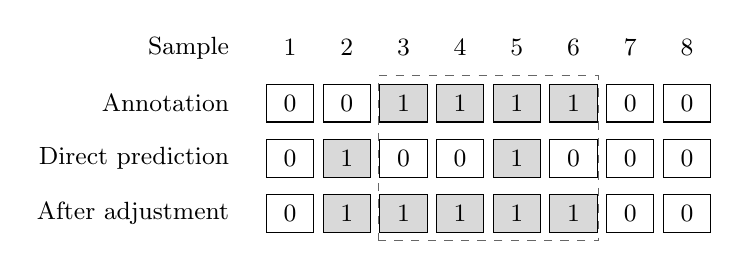
\begin{tikzpicture}[font=\small]
    \node[anchor=east] at (-.65,2.1) {Sample};
    \node[anchor=east] at (-.65,1.4) {Annotation};
    \node[anchor=east] at (-.65,.7) {Direct prediction};
    \node[anchor=east] at (-.65,0) {After adjustment};
    \foreach \j in {1,...,8}{
      \node at ({.72*(\j-1)},2.1) {\j};
    }
    \foreach \value [count=\j] in {0,0,1,1,1,1,0,0}{
      \pgfmathtruncatemacro{\shade}{15*\value}
      \node[draw,minimum width=.60cm,minimum height=.48cm,fill=black!\shade]
        at ({.72*(\j-1)},1.4) {\value};
    }
    \foreach \value [count=\j] in {0,1,0,0,1,0,0,0}{
      \pgfmathtruncatemacro{\shade}{15*\value}
      \node[draw,minimum width=.60cm,minimum height=.48cm,fill=black!\shade]
        at ({.72*(\j-1)},.7) {\value};
    }
    \foreach \value [count=\j] in {0,1,1,1,1,1,0,0}{
      \pgfmathtruncatemacro{\shade}{15*\value}
      \node[draw,minimum width=.60cm,minimum height=.48cm,fill=black!\shade]
        at ({.72*(\j-1)},0) {\value};
    }
    \draw[dashed,black!60] (1.12,-.35) rectangle (3.92,1.75);
  \end{tikzpicture}
  \caption{Illustrative point adjustment. The annotated positive interval
  comprises samples \num{3}--\num{6}. A direct hit at sample \num{5} gives
  credit for that whole interval, while the false alarm at sample \num{2}
  remains. The dashed boundary identifies the annotated interval.}
  \label{fig:datasets-pa}
\end{figure}

For the native benchmarks, positive intervals are contiguous runs in the
concatenated labels. For \ac{OPS-SAT}, adjustment respects fragment boundaries:
adjacent anomalous fragments are separate intervals. Each positive fragment
uses its repeated weak label. The exact native first-index convention is
retained for reproduction, while the fragment routine handles the first
sample of each fragment through an explicit nominal sentinel.
% Source: omnianomaly.adjust_predicts; opssat_pipeline.adjust_per_fragment.

Adjustment is an evaluation transformation, not a learned capability of
the model. It can assign credit before the first actual alarm and can
strongly increase recall on long intervals. The \ac{OPS-SAT} pointwise
counts additionally weight longer fragments more heavily. These properties
motivate reporting unadjusted score discrimination and fragment-level
metrics alongside the adjusted benchmark values. The adjustment is explicit
in the authors' code, although the TranAD+ article does not describe the
procedure in its evaluation-metrics section~\cite{TranADPlusReferenceCode,Yermakov2025TranADPlus}.

Two different quantities are commonly called \ac{ROC} area in the saved
reports. The continuous-score area evaluates the ordering of scores across
nominal and anomalous observations, without selecting a classification
threshold. The authors' implementation instead applies the area calculation
to binary predictions after adjustment. For a test set containing both
classes, the latter reduces to
\begin{equation}
  \mathrm{AUC}_{\mathrm{binary,adjusted}}
  =\frac{1}{2}\left(
      \frac{TP}{TP+FN}+\frac{TN}{TN+FP}
    \right).
  \label{eq:datasets-binary-auc}
\end{equation}
Here the confusion counts refer to adjusted point predictions. The two
terms are sensitivity and specificity, so this quantity is balanced
accuracy at one operating point. It is not the area obtained by ranking
the original continuous scores. The same distinction applies to the
continuous-score area computed from one score per \ac{OPS-SAT} fragment.

We also report average precision, calculated from the precision--recall
sequence induced by the score ranking. It is distinct from a trapezoidal
integral of that curve and depends on class prevalence. Table~\ref{tab:datasets-evaluations}
summarizes the evaluation paths used in the thesis. Their names and units
are retained in the result tables, rather than placing different quantities
under an unqualified AUC heading.

\begin{table}[htbp]
  \centering
  \small
  \begin{tabularx}{\textwidth}{@{}l*{3}{>{\raggedright\arraybackslash}X}@{}}
    \toprule
    Evaluation & Threshold or scoring choice & Labels used for selection & Reporting unit \\
    \midrule
    Original POT & Tail routine; best test-F1 alpha & Test labels for alpha and adjustment & Points after adjustment \\
    Original Best F1 & \num{200} thresholds; best test-F1 alpha & Test labels for threshold, alpha and adjustment & Points after adjustment \\
    Dense Best F1 & Distinct-score thresholds; best test-F1 alpha & Test labels for threshold, alpha and adjustment & Points after adjustment \\
    Fixed-score control & Alpha \num{0.5}; training-quantile threshold & None from test; training scores set threshold & Unadjusted points \\
    \acs{OPS-SAT} selection & Alpha, calibration and max/p95 aggregation & Validation fragment labels & Unadjusted fragment scores \\
    \bottomrule
  \end{tabularx}
  \caption{Evaluation paths. Alpha is absent for single-output models.
  Ranking metrics use continuous scores unless explicitly identified as
  binary-after-adjustment. \acs{OPS-SAT} pointwise paths use repeated weak
  fragment labels. The validation-selected fragment path is separate from
  the test-oracle searches.}
  \label{tab:datasets-evaluations}
\end{table}

\section{Computational cost and runtime measurements}
\label{sec:datasets-resources}
Resource assessment separates storage, arithmetic estimates and measured
execution time. Parameter counts include trainable weights and biases.
With \num{32}-bit floating-point parameters, their storage is
\begin{equation}
  M_{\theta}=4N_{\theta}\ \text{bytes},
  \label{eq:datasets-parameter-storage}
\end{equation}
where \(N_{\theta}\) is the number of stored parameter elements and
\(M_{\theta}\) is their memory in bytes. Buffers, intermediate activations
and optimizer states are separate quantities. A resumable checkpoint
contains more than the inference weights and is not used as a direct
estimate of deployed parameter storage.

Multiply--accumulate counts are analytical estimates for the implemented
matrix operations: attention projections and products, feed-forward maps
and the output linear layer. They exclude nonlinear functions, softmax,
elementwise operations and data movement. These estimates describe changes
in arithmetic demand; they are not measured energy consumption or a
complete hardware instruction count. Parameter sharing and pass removal
also have different effects: sharing a decoder reduces storage, whereas
removing a pass additionally avoids its execution.

Runtime is measured on the declared server platform. The architectural
campaign uses an NVIDIA A100 PCIe, \SI{40}{\giga\byte} model, with PyTorch
\texttt{2.8.0} and CUDA \texttt{12.8}. Parameters and operations use FP32, with
TensorFloat-32 disabled. Forward latency is measured at batch size
\num{1}, after \num{10} warm-up calls and over \num{100} timed calls.
CUDA synchronization brackets each measurement. The reported median,
mean and upper percentile describe those repeated calls for each run.
The earlier hyperparameter profiling uses \num{50} timed calls after the
same number of warm-ups; that difference is recorded with the results.
% Sources: resources.py measure, baselines.json; v10/v12 measurement_settings;
% v13/v14 manifest.execution (A100-PCIE-40GB, torch2.8.0+cu128, CUDA12.8).

The batch-one measurement includes host launch and synchronization overhead,
but excludes input transfer and anomaly-score calculation. Batched scoring
has a separate elapsed time including transfer and score production.
Training telemetry records epoch duration and peak allocated accelerator
memory. GPU-resident input caching can reduce transfer overhead while
retaining the batch order and numerical settings. It is recorded as part
of the execution configuration.

Repeated forward calls measure timing variation within a run; training
seeds measure variation across trained models. These sources of uncertainty
are reported separately. Measurements on this server do not establish
latency, power or memory feasibility on onboard processors or
\ac{FPGA} hardware~\cite{Sze2017EfficientDNN}.

\section{Reproducibility and experimental controls}
\label{sec:datasets-reproducibility}
The hyperparameter study combines the window-size and feed-forward grids
from two recorded campaigns. For each dataset, it contains \num{6} window
lengths and \num{5} feed-forward widths, with seeds
\num{2026}, \num{2027} and \num{2028}. Effective integer dimensions are
used when matching settings. The architectural study evaluates the
reference, shared-decoder, single-pass and encoder-only implementations
at the four settings in Table~\ref{tab:datasets-study-settings}, using
seeds \num{2026}--\num{2030}. Model definitions and changes in objectives
are discussed in Chapter~\ref{chap:architecture}.

A common seed fixes the initial state of the random-number generators.
Architectures with different computation graphs need not share corresponding
parameter values or optimizer trajectories. The main study reports means
and sample standard deviations across the declared seeds. The dataset split
is fixed, so seed variation does not measure uncertainty due to acquiring
a different telemetry sample.
% Sources: results/analysis_v10_v12/runs_270.csv; configs/baselines.json;
% tranad_variants/configs/campaigns/additional.json; v13 profile manifests.

Each experiment records its configuration, input-file hashes, source hashes,
execution environment and checkpoint origin. Model and optimizer state,
learning-rate scheduler state and random-generator state are saved for
recovery. Continued-training controls start from the completed
\num{50}-epoch recovery state and run to a fixed \num{100}-epoch endpoint.
They retain the scheduler and absolute epoch index in the loss, rather
than restarting either. The source experiment remains unchanged and the
continued result is stored separately.

Evaluation controls reuse stored scores or frozen checkpoints. They can
compare threshold searches, remove padded target copies, or perturb the
past while retaining the current reconstruction target. These are diagnostic
comparisons, not new training samples. Their selection rules and scoring
settings are declared before interpreting the examples or differences.
They do not replace the aggregate test evaluation.

Comparisons across campaigns are checked for preprocessing, label alignment,
score definition and numerical implementation. Source hashes alone identify
a difference; they do not prove numerical agreement or disagreement. Boundary
cases and saved-score checks are therefore documented with the relevant
comparison in Chapters~\ref{chap:replication} and~\ref{chap:ablation}.
Complete identifiers, configuration records and execution commands belong
in Appendix~\ref{app:reproducibility}. This provenance allows model changes
to be distinguished from changes in the data or evaluation procedure.
